%%%%%%%%%%%%%%%%%%%%%%%%%%%%%%%%%%%%%%%%%%%%%%%%%%%%%%%%%%%%%%%%%%%%%%%%%%%%%%%%%%%%%%%%%%%%%%%%%%%%%%%%%%%%%%%%%%%%%%%%%%%%%%%%%%%%%%%%%%%%%%%%%%%%%%%%%%%%%%%%%%%%%%%%%%%%%%%%%%%%%%%%%%%%
% Written By Michael Brodskiy
% Class: Differential Equations (MATH-294)
% Professor: M. Shah
%%%%%%%%%%%%%%%%%%%%%%%%%%%%%%%%%%%%%%%%%%%%%%%%%%%%%%%%%%%%%%%%%%%%%%%%%%%%%%%%%%%%%%%%%%%%%%%%%%%%%%%%%%%%%%%%%%%%%%%%%%%%%%%%%%%%%%%%%%%%%%%%%%%%%%%%%%%%%%%%%%%%%%%%%%%%%%%%%%%%%%%%%%%%

\documentclass[12pt]{article} 
\usepackage{alphalph}
\usepackage[utf8]{inputenc}
\usepackage[russian,english]{babel}
\usepackage{titling}
\usepackage{amsmath}
\usepackage{graphicx}
\usepackage{enumitem}
\usepackage{amssymb}
\usepackage[super]{nth}
\usepackage{everysel}
\usepackage{ragged2e}
\usepackage{geometry}
\usepackage{fancyhdr}
\usepackage{cancel}
\usepackage{siunitx}
\geometry{top=1.0in,bottom=1.0in,left=1.0in,right=1.0in}
\newcommand{\subtitle}[1]{%
  \posttitle{%
    \par\end{center}
    \begin{center}\large#1\end{center}
    \vskip0.5em}%

}
\usepackage{hyperref}
\hypersetup{
colorlinks=true,
linkcolor=blue,
filecolor=magenta,      
urlcolor=blue,
citecolor=blue,
}

\urlstyle{same}


\title{Undetermined Coefficients $-$ Superposition Approach}
\date{\today}
\author{Michael Brodskiy\\ \small Professor: Meetal Shah}

% Mathematical Operations:

% Sum: $$\sum_{n=a}^{b} f(x) $$
% Integral: $$\int_{lower}^{upper} f(x) dx$$
% Limit: $$\lim_{x\to\infty} f(x)$$

\begin{document}

\maketitle

\begin{itemize}

  \item Method of Undetermined Coefficients $-$ A way of obtaining a particular solution to a nonhomogeneous equation. 

  \item Ex. $y''+4y'-2y=2x^2-3x+6$

    \begin{enumerate}

      \item First solve the associated homogeneous equation.

      \item Next, Assume the particular solution, $y_p$, is a quadratic (as the DE equals a quadratic): 

        $$y_p'=2Ax+B,\,y_p''=2A$$
        $$2A+8Ax+4B-2Ax^2-2Bx-2C=2x^2-3x+6$$
        $$A=-1,\,B&=-\frac{5}{2},\,C=-9$$
        $$\therefore y_p=-x^2-\frac{5}{2}x-9$$

      \item Then, find the complementary solution and add them together:

        $$y=y_c+y_p=c_1e^{-(2+\sqrt{6})x}+c_2e^{(-2+\sqrt{6})x}-x^2-\frac{5}{2}x-9$$

    \end{enumerate}

  \item The form of a prediction may be found using the following table:\footnote{Note: for functions like $8xe^{2x}$, it is necessary to create a second term, $(Ax+B)e^{2x}+e^{2x}$}

    \begin{figure}[h]
      \centering
      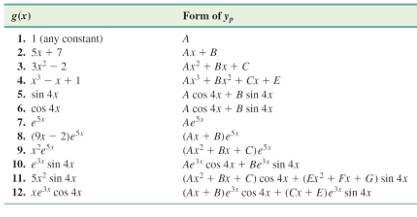
\includegraphics{Figures/TrialTable.png}
      \caption{Table of Trials}
      \label{fig:1}
    \end{figure}

  \item If any $y_p$ predictions are similar to terms in the complementary function, multiply by $x^n$, where $n$ is the smallest integer which eliminates any correlation to the complementary function. 

\end{itemize}

\end{document}

